\part{Linear Algebra}
\chapter{Vectors}
\section{Coordinate Space and the Algebra of Vectors}
\begin{definition}
By a \vocab{vector} we will mean a list of $n$ real numbers $x_1,x_2,\dots,x_n$ where $n$ is a positive integer. Mostly this list will be written as a row vector:
\[ (x_1,x_2,\dots,x_n) \]
Sometimes the numbers will be arranged as a coluumn vector:
\[ \begin{pmatrix}
x_1\\x_2\\\vdots\\x_n
\end{pmatrix} \]
Often we will denote such a vector by a single letter in bold, say $\vb{x}$, and refer to $x_i$ as the $i$-th coordinate of $\vb{x}$.
\end{definition}

\begin{definition}
For a given $n$, we denote the set of all vectors with $n$ coordinates as $\RR^n$, and often refer to $\RR^n$ as $n$-dimensional coordinate space or simply as $n$-dimensional space. If $n=2$ then we commonly use $x$ and $y$ as coordinates and refer to $\RR^2=\{(x,y)\mid x,y\in\RR\}$ as the $xy$-plane. If $n=3$ then we commonly use $x$, $y$ and $z$ as coordinates and refer to $\RR^3=\{(x,y,z)\mid x,y,z\in\RR\}$ as $xyz$-space.
\end{definition}

\begin{definition}
There is a special vector $(0,0,\dots,0)$ in $\RR^n$ which we denote as $\vb{0}$ and refer to as the \vocab{zero vector}.
\end{definition}

A vector is an object that has both magnitude and direction. In simple terms, especially when we are thinking of $\RR^2$ or $\RR^3$, a vector is an arrow.

\begin{definition}
The points $(0,0,\dots,0,x_i,0,\dots,0)$ in $\RR^n$, where $x_i$ is a real number, comprise the $x_i$-axis, with the origin lying at the intersection of all the axes.
\end{definition}

Given two vectors $\vb{u}=(u_1,u_2,\dots,u_n)$ and $\vb{v}=(v_1,v_2,\dots,v_n)$ in $\RR^n$, we can add and subtract them much as you would expect, by separately adding the corresponding coordinates; that is, 
\[ \vb{u}+\vb{v}=(u_1+v_1,u_2+v_2,\dots,u_n+v_n); \quad \vb{u}-\vb{v}=(u_1-v_1,u_2-v_2,\dots,u_n-v_n). \]

\begin{remark}
Note that two vectors may be added if and only if they have the same number of coordinates. No immediate sense can be made of adding a vector in $\RR^2$ to one from $\RR^3$, for example.
\end{remark}

Given a vector $\vb{v}=(v_1,v_2,\dots,v_n)$ and a real number $k$ then the scalar multiple $k\vb{v}$ is defined as
\[ k\vb{v}=(kv_1,kv_2,\dots,kv_n). \]

\begin{definition}
The $n$ vectors
\[ (1,0,\dots,0), \quad (0,1,0,\dots,0), \quad \dots, \quad (0,\dots,0,1,0), \quad (0,\dots,0,1) \]
in $\RR^n$ are known as the \vocab{standard} (or canonical) basis for $\RR^n$. We will denote these, respectively, as $\vb{e}_1,\vb{e}_2,\dots,\vb{e}_n$.
\end{definition}

\begin{notation}
When $n=2$, the vectors $(1,0)$ and $(0,1)$ form the standard basis for $\RR^2$. These are also commonly denoted by the symbols $\vb{i}$ and $\vb{j}$ respectively. Note that any vector $\vb{v}=(x,y)$ can be written uniquely as a linear combination of $\vb{i}$ and $\vb{j}$: that is $(x,y)=x\vb{i}+y\vb{j}$ and this is the only way to write $(x,y)$ as a sum of scalar multiples of $\vb{i}$ and $\vb{j}$.

When $n=3$, the vectors $(1,0,0)$, $(0,1,0)$, $(0,0,1)$ form the standard basis for $\RR^3$ being respectively denoted $\vb{i}$, $\vb{j}$, $\vb{k}$.
\end{notation}

\section{The Geometry of Vectors}
\begin{definition}
The \vocab{length} (or \vocab{magnitude}) of a vector $\vb{v}=(v_1,v_2,\dots,v_n)$, which is written $|\vb{v}|$, is defined by
\[ |\vb{v}|=\sqrt{v_1^2+v_2^2+\cdots+v_n^2}. \]
We say a vector $\vb{v}$ is a \vocab{unit vector} if it has length $1$.
\end{definition}

This formula formalises our intuitive idea of a vector as an arrow having a length; the length of the arrow is exactly what you'd expect it to be from Pythagoras’ Theorem. We see this is the distance of the point $\vb{v}$ from the origin, or equivalently the distance a point moves when it is translated by $\vb{v}$. So if $\vb{p}$ and $\vb{q}$ are points in $\RR^n$, then the vector that will translate $\vb{p}$ to $\vb{q}$ is $\vb{q}-\vb{p}$, and hence we define:

\begin{definition}
The distance between two points $\vb{p}$ and $\vb{q}$ in $Rn$ is $|\vb{q}-\vb{p}|$ (or equally $|\vb{p}-\vb{q}|$). In terms of their coordinates $p_i$ and $q_i$ we have
\[ \text{distance between }\vb{p}\text{ and }\vb{q}=\sqrt{\sum_{i=0}^n(p_i-q_i)^2}. \]
\end{definition}

Note that $|\vb{v}|>0$ and that $|\vb{v}|=0$ if and only if $\vb{v}=\vb{0}$.

Also $|\lambda\vb{v}|=|\lambda||\vb{v}|$ for any real number $\lambda$.

\begin{proposition}[Triangle Inequality]
Let $\vb{u}$ and $\vb{v}$ be vectors in $\RR^n$. Then
\begin{equation}
|\vb{u}+\vb{v}|\le|\vb{u}|+|\vb{v}|.
\end{equation}
If $\vb{v}\neq\vb{0}$ then equality holds if and only if $\vb{u}=\lambda\vb{v}$ for some $\lambda\ge0$.
\end{proposition}

Geometrically, this is intuitively obvious.

\begin{proof}
Let $\vb{u}=(u_1,u_2,\dots,u_n)$ and $\vb{v}=(v_1,v_2,\dots,v_n)$. The inequality is trivial if $\vb{v}=0$, so suppose $\vb{v}\neq\vb{0}$. Note that for any real number $t$,
\[ 0\le|\vb{u}+t\vb{v}|^2=\sum_{i=1}^n(u_i+tv_i)^2=|\vb{u}|^2+2t\sum_{i=1}^nu_iv_i+t^2|\vb{v}|^2. \]
As $|\vb{v}|\neq0$, the RHS of the above inequality is a quadratic in $t$ which is always non-negative, and thus has non-positive discriminant ($b^2\le4ac$). Hence
\[ 4\brac{\sum_{i=0}^nu_iv_i}^2\le4|\vb{u}|^2|\vb{v}|^2 \quad \text{giving} \quad \absolute{\sum_{i=1}^nu_iv_i}\le|\vb{u}||\vb{v}|. \]
Finally

\end{proof}

\chapter{Linear Systems and Matrices}
\section{Systems of linear equations}
\begin{definition}
By a \vocab{linear system}, or \vocab{linear system of equations}, we will mean a set of $m$ simultaneous equations in $n$ real variables $x_1,x_2,\dots,x_n$ which are of the form
\begin{equation}\label{eqn:linear_system}
\begin{cases}
a_{11}x_1+a_{12}x_2+\cdots+a_{1n}x_n&=b_1 \\
a_{21}x_1+a_{22}x_2+\cdots+a_{2n}x_n&=b_2 \\
&\vdots \\
a_{m1}x_1+a_{m2}x_2+\cdots+a_{mn}x_n&=b_m
\end{cases}
\end{equation}
\[  \]
where $a_{ij}$ and $b_i$ are real constants.
\end{definition}

Any vector $(x_1,x_2,\dots,x_n)$ which satisfies \cref{eqn:linear_system} is said to be a \vocab{solution}; if the linear system has one or more solutions then it is said to be \vocab{consistent}. The \vocab{general solution} to the system is any description of all the solutions of the system. We will see later that such linear systems can have zero, one or infinitely many solutions.

We will often write the linear system \cref{eqn:linear_system} as the \vocab{augmented matrix} $(A\mid\vb{b})$ where
\[ A=\begin{pmatrix}
    a_{11} & a_{12} & \cdots & a_{1n} \\
    a_{21} & a_{22} & \cdots & a_{2n} \\
    \vdots & \vdots & & \vdots \\ 
    a_{m1} & a_{m2} & \cdots & a_{mn}
\end{pmatrix} \quad \text{and} \quad 
\vb{b}=\begin{pmatrix}b_1\\b_2\\\vdots\\b_m\end{pmatrix}. \]
For now, we won't consider a matrix (such as $A$) or vector (such as $\vb{b}$) to be anything more than an array of numbers.

To solve systems of linear equations efficiently, we introduce such a process called \vocab{row-reduction}. It relies on three types of operation, called elementary row operations (EROs), which importantly do not affect the set of solutions of a linear system as we apply them.

\begin{definition}
Given a linear system of equations, an \vocab{elementary row operation} (ERO) is an operation of one of the following three kinds.
\begin{enumerate}[label=(\alph*)]
\item Swap two equations.
\item Multiply an equation by a non-zero constant.
\item Add a multiple of one equation to another equation.
\end{enumerate}
\end{definition}

\begin{notation} \
\begin{enumerate}[label=(\alph*)]
\item Let $S_{ij}$ denote the ERO which swaps rows $i$ and $j$ (or equivalently the $i$-th and $j$-th equations).
\item Let $M_i(\lambda)$ denote the ERO which multiplies row $i$ by $\lambda\neq0$ (or equivalently both sides of the ith equation).
\item For $i\neq j$, let $A_{ij}(\lambda)$ denote the ERO which adds $\lambda$ times row $i$ to row $j$ (or does the same to the equations).
\end{enumerate}
Note this is not standard notation in any way, but I have introduced it here for
convenience.
\end{notation}

\section{Matrices and matrix algebra}
At its simplest, a matrix is just a two-dimensional array of numbers.

\begin{definition}
Let $m$ and $n$ be positive integers. An $m\times n$ \vocab{matrix} is an array of real numbers arranged into $m$ rows and $n$ columns.
\end{definition}

The numbers in a matrix are its \vocab{entries}. Given an $m\times n$ matrix $A$, we will write $a_{ij}$ for the entry in the $i$-th row and $j$-th column. Note that $i$ can vary between $1$ and $m$, and that $j$ can vary between $1$ and $n$. So
\[ i\text{-th row}=(a_{i1},\dots,a_{in}) \quad \text{and} \quad j\text{-th column}=\begin{pmatrix}a_{ij}\\\vdots\\a_{mj}\end{pmatrix} \]

\begin{notation}
We shall denote the set of real $m\times n$ matrices as $M_{mn}$. Note that $M_{1n}=\RR^n$ and that $M_{n1}=\RR^n_\text{col}$.
\end{notation}

There are three important operations that can be performed with matrices: matrix addition, scalar multiplication and matrix multiplication. As with vectors, not all pairs of matrices can be meaningfully added or multiplied.

\textbf{Addition}: Let $A=(a_{ij})$ be an $m\times n$ matrix (recall: $m$ rows and $n$ columns) and $B=(b_{ij})$ be a $p\times q$ matrix. As with vectors, matrices are added by adding their corresponding entries. So, as with vectors, to add two matrices they have to be the same size -- that is, to add $A$ and $B$, we must have $m=p$ and $n=q$. If we write $C=A+B=(c_{ij})$ then $c_{ij}=a_{ij}+b_{ij}$ for $1\le i\le m$ and $1\le j\le n$.

In general, matrix addition is commutative as for matrices $M$ and $N$ of the same size we have
\[ M+N=N+M. \]
Addition of matrices is also associative as
\[ L+(M+N)=(L+M)+N \]
for any matrices of the same size.

\begin{definition}
The $m\times n$ \vocab{zero matrix} is the matrix with $m$ rows and $n$ columns whose every entry is $0$. This matrix is simply denoted as $0$ unless we need to specify its size, in which case it is written $0_{mn}$.
\end{definition}

A simple check shows that $A+0_{mn}=A=0_{mn}+A$ for any $m\times n$ matrix $A$.

\textbf{Scalar multiplication}: Let $A=(a_{ij})$ be an $m\times n$ matrix and $k$ be a real number (a scalar). Then the matrix $kA$ is defined to be the $m\times n$ matrix with $(i,j)$-th entry equal to $ka_{ij}$.

More generally the following identities hold. Let $A$, $B$, $C$ be $m\times n$ matrices and $\lambda,\mu$ be real numbers.
\begin{itemize}
\item $A+0_{mn}=A$
\item $A+B=B+A$
\item $0A=0_{mn}$
\item $A+(-A)=0_{mn}$
\item $(A+B)+C=A+(B+C)$
\item $1A=A$
\item $(\lambda+\mu)A=\lambda A+\mu A$
\item $\lambda(A+B)=\lambda A+\lambda B$
\item $\lambda(\mu A)=(\lambda\mu)A$
\end{itemize}
These are readily verified and show that $M_{mn}$ is a real vector space.

Based on how we added matrices then you might think that we multiply matrices in a similar fashion, namely multiplying corresponding entries, but we do not. At first glance the rule for multiplying matrices is going to seem rather odd but, in due course, we will see why matrix multiplication is done as follows and that this is natural in the context of matrices representing linear maps.

\textbf{Matrix multiplication}: We can multiply an $m\times n$ matrix $A=(a_{ij})$ with an $p\times q$ matrix $B=(b_{ij})$ if $n=p$. That is, $A$ must have as many columns as $B$ has rows. If this is the case then the product $C=AB$ is the $m\times q$ matrix with entries
\begin{equation}
c_{ij}=\sum_{k=1}^n a_{ik}b_{kj}
\end{equation}
for $1\le i\le m$ and $1\le j\le q$.

It may help to write the rows of $A$ as $\vb{r}_1,\dots,\vb{r}_m$ and the columns of $B$ as $\vb{c}_1,\dots,\vb{c}_q$. Then the above equation is equivalent to
\[ \text{the }(i,j)\text{-th entry of }AB=\vb{r}_i\cdot\vb{c}_j \]
for $1\le i\le m$ and $1\le j\le q$.

\begin{definition}
The $n\times n$ \vocab{identity matrix} $I_n$ is the $n\times n$ matrix with entries
\[ \delta_{ij}=\begin{cases}
1 & \text{if }i=j \\
0 & \text{if }i\neq j
\end{cases}. \]
\end{definition}

The identity matrix will be simply denoted as $I$ unless we need to specify its size. The $(i,j)$-th entry of $I$ is denoted as $\delta_{ij}$ which is referred to as the \textbf{Kronecker delta}.

\todo{remove below}


Matrices: linear transformations, kernels and images; inner products, inner product spaces, orthonormal sets, and the Gram-Schmidt process; eigenvectors and eigenvalues; matrix diagonalisation and its applications; symmetric and Hermitian matrices; quandratic forms and bilinear forms; Jordan normal form and other canonical forms.

• determinant of a square matrix and inverse of a non-singular matrix (2 × 2 and 3 × 3 matrices only)
• use of matrices to solve a set of linear equations (including row reduction and echelon forms, and geometrical interpretation of the solution)

Here are some special matrices:
\begin{itemize}
\item \textbf{Square matrix} of order $n$ is a matrix with $n$ rows and $n$ columns, i.e. \# rows = \# columns
\[ \mathbf{A} = \begin{bmatrix}
    a_{11} & a_{12} & \cdots & a_{1m} \\
    a_{21} & a_{22} & \cdots & a_{2m} \\
    \vdots & \vdots & \ddots & \vdots \\
    a_{m1} & a_{m2} & \cdots & a_{mm}
\end{bmatrix} \]

\item \textbf{Diagonal matrix}
\[ \mathbf{A} = \begin{bmatrix}
    a_{11} & 0 & \cdots & 0 \\
    0 & a_{22} & \cdots & 0 \\
    \vdots & \vdots & \ddots & \vdots \\
    0 & 0 & \cdots & a_{mm}
\end{bmatrix} \]

\item \textbf{Symmetric matrix}
\[ \mathbf{A} = \mathbf{A}^T \]

\item \textbf{Row matrix}: matrix with only one row (sometimes used to represent a vector)
\[ \mathbf{A} = 
\begin{bmatrix}
    a_{11} & a_{12} & \cdots & a_{1n}
\end{bmatrix} \]

\item \textbf{Column matrix}:  matrix with only one column (sometimes used to represent a vector)
\[ \mathbf{A} = 
\begin{bmatrix}
    a_{11} \\
    a_{21} \\
    \vdots \\
    a_{m1}
\end{bmatrix} \]
\end{itemize}

Conjugate matrix

\subsection{Identity Matrix, Determinant and Inverse of a Matrix}
\subsubsection{Identity Matrix}
The identity matrix has the property that when multiplied with another matrix it leaves the other matrix unchanged:
\begin{equation}
\mathbf{AI} = \mathbf{A} = \mathbf{IA}
\end{equation}

\subsubsection{Transpose of Matrix}
The \vocab{transpose} of an $m \times n$ matrix $\mathbf{A}$ is the $n \times m$ matrix $\mathbf{A}^T$ formed by turning rows into columns and vice versa:
\[ (\mathbf{A}^T)_{i,j} = \mathbf{A}_{j,i} \]
For example:
\[ \begin{bmatrix}
    1 & 2 & 3 \\
    0 & -6 & 7
\end{bmatrix}^T =
\begin{bmatrix}
    1 & 0 \\
    2 & -6 \\
    3 & 7
\end{bmatrix} \]

\subsubsection{Determinant of Matrix}
The \vocab{determinant} of a $2 \times 2$ matrix $\mathbf{A}$, denoted by $|\mathbf{A}|$ or $\det\mathbf{A}$, is
\[ \begin{vmatrix}
    a & b\\
    c & d
\end{vmatrix} = ad-bc \]
and the determinant of a $3 \times 3$ matrix is
\[ \begin{vmatrix}
    a_{11} & a_{12} & a_{13}\\ 
    a_{21} & a_{22} & a_{23}\\
    a_{31} & a_{32} & a_{33} 
\end{vmatrix}
= a_{11}\begin{vmatrix} 
    a_{22} & a_{23} \\ 
    a_{32} & a_{33}
\end{vmatrix} 
+ a_{12}\begin{vmatrix}
    a_{23} & a_{21} \\ 
    a_{33} & a_{31}
\end{vmatrix} 
+ a_{13}\begin{vmatrix}
    a_{21} & a_{22} \\
    a_{31} & a_{32}
\end{vmatrix}
 \]

More generally, for a $n \times n$ matrix $\mathbf{A}$, the formal method is as follows. First we will require some definitions:
\begin{itemize}
\item The $(i,j)$-\textbf{minor} of $\mathbf{A}$ is the determinant of the submatrix obtained by deleting the $i$-th row and $j$-th column of $\mathbf{A}$. We denote this submatrix as $M_{ij}(\mathbf{A})$.
\item The $(i,j)$-\textbf{cofactor} of $\mathbf{A}$ is the matrix $C_{ij}(\mathbf{A})=(-1)^{i+j}M_{ij}(\mathbf{A})$.
\end{itemize}
Now, in order to calculate the determinant of an $n \times n$ matrix $\mathbf{A}$, we calculate
\begin{equation}
|\mathbf{A}| = \sum_{i=1}^n a_{1n}C_{1n}(\mathbf{A}) = a_{11}C_{11}(\mathbf{A}) + a_{12}C_{12}(\mathbf{A}) + a_{13}C_{13}(\mathbf{A}) + \cdots + a_{1n}C_{1n}(\mathbf{A})
\end{equation}

A matrix whose determinant is zero, i.e. $|\mathbf{A}| = 0$, is said to be \vocab{singular}; a matrix whose determinant is non-zero, i.e. $|\mathbf{A}| \neq 0$, is said to be \vocab{non-singular}.

\subsubsection{Inverse of Matrix}
Only non-singular matrices have an inverse matrix. The \vocab{inverse} of a matrix $\mathbf{A}$ is denoted $\mathbf{A}^{-1}$ and has the following property:
\begin{equation}
\mathbf{AA}^{-1} = \mathbf{A}^{-1}\mathbf{A} = \mathbf{I}
\end{equation}

To find the inverse of a 2 × 2 matrix $\mathbf{A}$ given by
\[ \mathbf{A} = \begin{bmatrix}
    a & b \\
    c & d
\end{bmatrix} \]
we have the following formula:
\begin{equation}
\mathbf{A}^{-1} = \frac{1}{|\mathbf{A}|}\begin{bmatrix} d & -b \\ -c & a \end{bmatrix}
\end{equation}
where $|\mathbf{A}|=ad-bc\neq0$.

\begin{remark}
There exists more complicated methods for finding the inverses of $3 \times 3$ matrices and square matrices of larger size, which we will not discuss here.
\end{remark}

\subsection{Rank of Matrix}

\subsection{Orthogonal Matrix}
A square matrix $A$ is called \textbf{orthogonal} if
\[ \mathbf{A}\mathbf{A}^T = \mathbf{I} \text{ and } \mathbf{A}^T\mathbf{A} = \mathbf{I}. \]

Show that if $\mathbf{A}$ and $\mathbf{B}$ are orthogonal matrices, then $\mathbf{AB}$ is an orthogonal matrix.

\subsection{System of Linear Equations}
\begin{exmp}{}{}
Solve the following linear system by performing elementary row operations:
\begin{align*}
x - 3y &= 2 \\
-x + y + 5z &= 2 \\
2x - 5y + z &= 0
\end{align*}
\end{exmp}

\begin{proof}[Solution]
The augmented matrix of the linear system is
\[ \begin{bmatrix}
    1 & -3 & 0 & 2 \\
    -1 & 1 & 5 & 2 \\
    2 & -5 & 1 & 0
\end{bmatrix} \]

Hence
\begin{figure}[H]
    \centering
    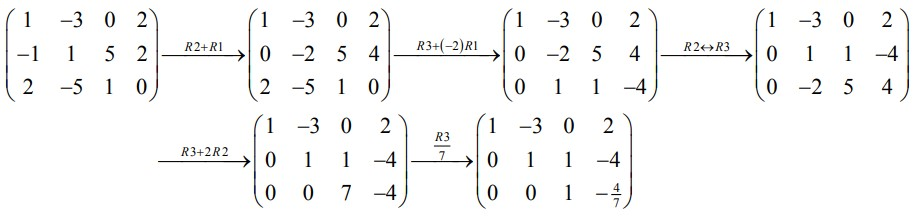
\includegraphics[width=16cm]{images/aug_matrix.jpg}
\end{figure}

By backward substitution, we obtain the solution of the linear system:
\[ x=-\frac{58}{7}, \quad y=-\frac{24}{7}, \quad z=-\frac{4}{7}. \]
\end{proof}

Consider the following two linear systems:
\begin{equation*}\tag{1}
\begin{split}
x + 2y - z + 5w &= -1 \\
y + 3z - w &= 2 \\
z + 2w &= 3 \\
w &= 1
\end{split}
\end{equation*}
and
\begin{equation*}\tag{2}
\begin{split}
x &= 3 \\
y &= 1 \\
z &= 2 \\
w &= 5
\end{split}
\end{equation*}
The solution to (1) can be obtained by backward substitution, while the solution to (2) is immediate.

The augmented matrices of the linear systems (1) and (2) are respectively
\[ \begin{bmatrix}
    1 & 2 & -1 & 5 & -1 \\
    0 & 1 & 3 & -1 & 2 \\
    0 & 0 & 1 & 2 & 3 \\
    0 & 0 & 0 & 1 & 1
\end{bmatrix} \quad \text{and} \quad
\begin{bmatrix}
    1 & 0 & 0 & 0 & 3 \\
    0 & 1 & 0 & 0 & 1 \\
    0 & 0 & 1 & 0 & 2 \\
    0 & 0 & 0 & 1 & 5
\end{bmatrix} \]
The first matrix is an example of a matrix in \textbf{row-echelon form}, while the second matrix is an example of a matrix in \textbf{reduced row-echelon form}.

\begin{defn}{Row-echelon form}{}
A matrix is said to be in \textbf{row-echelon form} if it satisfies all the following properties:
\begin{enumerate}
\item If there are any rows that consist entirely of zeros, then they are grouped together at the bottom of the matrix.
\item If a row does not consist of entirely of zeros, then the first nonzero number in the row is a 1. We call this a leading 1.
\item In any two successive rows that do not consists entirely of zeros, the leading 1 in the lower row occurs further to the right than the leading 1 in the higher row.
\end{enumerate}
The matrix is said to be in \textbf{reduced row-echelon form} if, in addition to the above three properties, the following property is satisfied:
\begin{enumerate}[resume]
\item Each column that contains a leading 1 has zeros everywhere else in that column.
\end{enumerate}
\end{defn}

\begin{exmp}{Linear system with a unique solution}{} 
The augmented matrix of a linear system in $(x,y,z)$ has been reduced to the given row-echelon form:
\[ \begin{bmatrix}
    1 & 2 & -1 & 2 \\
    0 & 1 & 3 & -1 \\
    0 & 0 & 1 & 4
\end{bmatrix} \]
Solve the linear system.
\end{exmp}

\begin{proof}[Solution]
The corresponding linear system is
\begin{align*}
x + 2y - z &= 2 \\
y + 3z &= -1 \\
z &= 4
\end{align*}
By backward substitution, we obtain the solution $x=32$, $y=-13$ and $z=4$.
\end{proof}

\begin{exmp}{Linear system with infinitely many solutions}{}
Write down all the solutions of 
\[ x+2y-z=3. \]
\end{exmp}

\begin{proof}[Solution]
Let $y=s$ and $z=t$, then $x=3-2s+t$.

Thus all the solutions are $x=3-2s+t$, $y=s$ and $z=t$, where $s,t\in\RR$.
\end{proof}

\begin{remark}
Note that $s$ and $t$ are called \textbf{parameters}, and the set of all solutions expressed in terms of the parameters is called the \textbf{general solution} of the linear system.
\end{remark}

\begin{exmp}{}{}
The augmented matrix of a linear system in $(x,y,z,w)$ has been reduced to the reduced-row echelon form:
\[ \begin{bmatrix}
    1 & 0 & 0 & 2 & -7 \\
    0 & 1 & 0 & 1 & 5 \\
    0 & 0 & 1 & 3 & 1 \\
    0 & 0 & 0 & 0 & 0
\end{bmatrix} \]
Solve the linear system.
\end{exmp}

\begin{proof}[Solution]
The corresponding linear system is
\begin{align*}
x + 2w &= -7 \\
y + w &= 5 \\
z + 3w &= 1
\end{align*}
The variables (unknowns) that corresponding to the leading 1's, namely $x$, $y$ and $z$, are called \textbf{leading variables}. The non-leading variables ($w$ in this case) are called \textbf{free variables}.

Solving for leading variables in terms of variables, we can assign any arbitrary value to the free variable $w$, say $t$, which then determines the values of the leading variable. Thus this linear system has \emph{infinitely many solutions} given by
\[ x=-7-2t, \quad y=5-t, \quad z=1-3t, \quad w=t \quad \text{where } t\in\RR \]
\end{proof}

\begin{defn}{Gaussian elimination}{}
The method of solving a linear system by reducing the corresponding augmented matrix to row-echelon form (respectively reduced row-echelon form) is unknown as \textbf{Gaussian elimination} (respectively \textbf{Gauss-Jordan elimination}).
\end{defn}

\begin{exmp}{}{}
Without using a calculator, solve the linear system
\begin{align*}
3x + 4y - 2z + 13w &= 9 \\
x + 2y - 2z + 7w &= 5 \\
2x + y + 4z + 6w &= -3
\end{align*}
\end{exmp}

\begin{proof}[Solution]
We write down the augmented matrix of the linear system and then perform elementary row operations to reduce it to row-echelon form or reduced row-echelon form:
\begin{figure}[H]
    \centering
    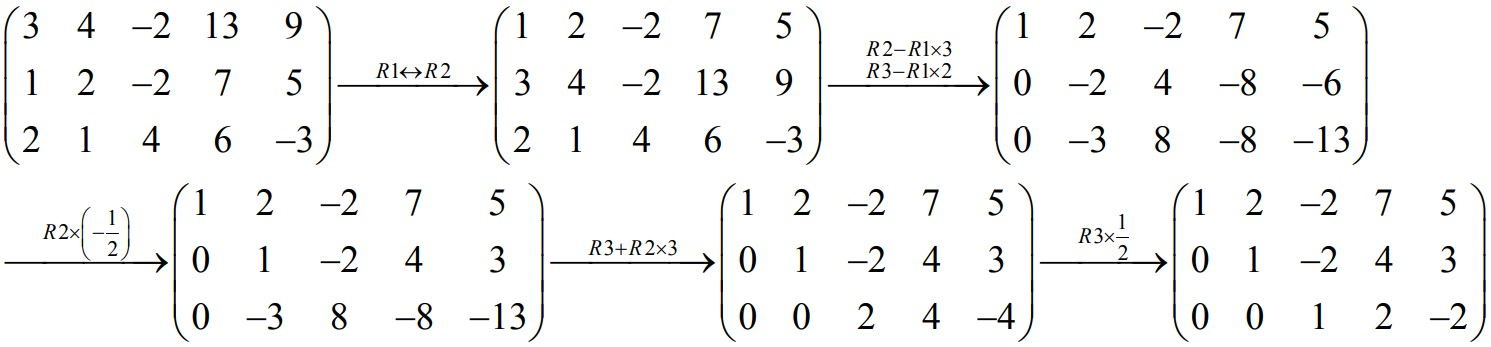
\includegraphics[width=16cm]{images/matrix_1.jpg}
\end{figure}
The linear system corresponding to the row-echelon form is
\begin{align*}
x + 2y - 2z + 7w &= 5 \\
y - 2z + 4w &= 3 \\
z + 2w &= -2
\end{align*}
which has the same set of solutions as the given linear system. Now $x$, $y$ and $z$ are the leading variables, and $w$ is the free variable. Let $w=t$ where $t\in\RR$ is an arbitrary number. By backward substitution, $z=-2-2t, y=-1-8t, x=3+5t$. Thus the general solution of the given linear system is
\[ x=3+5t, \quad y=-1-8t, \quad z=-2-2t, \quad w=t \quad \text{where } t\in\RR \]
Alternatively, we can further reduce the row-echelon form to reduced row-echelon form, then assign $w=t$ to obtain the same general solution.
\end{proof}

\begin{exmp}{Geometrical interpretation}{}
The general solution of the system of linear equations
\begin{align*}
x + y &= -1 \\
2x + y + z &= 3 \\
x + z &= 4
\end{align*}
is given by $x=4-t, y=-5+t, z=t$. What is the geometrical interpretation of the solution?
\end{exmp}

\begin{proof}[Solution]
The three planes $x+y=-1$, $2x+y+z=3$ and $x+z=4$ intersect in a common line, with vector equation
\[ r = \begin{pmatrix} x \\ y \\ z \end{pmatrix} 
= \begin{pmatrix} 4-t \\ -5+t \\ t \end{pmatrix} 
= \begin{pmatrix} 4 \\ -5 \\ 0 \end{pmatrix} + t\begin{pmatrix} -1 \\ 1 \\ 1 \end{pmatrix}, \quad t\in\RR \]
\end{proof}

\subsubsection{Homogenous Linear Systems}
\begin{defn}{Homogenous linear system}{}
A linear system of the form
\[ \begin{split}
a_{11}x_1 + a_{12}x_2 + \cdots + a_{1n}x_n &= 0 \\
a_{21}x_1 + a_{22}x_2 + \cdots + a_{2n}x_n &= 0 \\
&\vdots \\
a_{m1}x_1 + a_{m2}x_2 + \cdots + a_{mn}x_n &= 0
\end{split} \]
is known as a \textbf{homogeneous linear system}.
\end{defn}

Every homogeneous linear system is consistent, since $x_1=x_2=\cdots=x_n=0$ is a solution; this solution is called the \textbf{trivial solution}; if there are other solutions, then they are called \textbf{non-trivial solutions}, i.e. a solution $x_1=s_1, x_2=s_2, \dots, x_n=s_n$ is a non-trivial solution if \emph{at least one} of $s_i \neq 0$.

\begin{thrm}{}{}
Every homogeneous system of linear equations with more unknowns than equations has infinity many solutions.
\end{thrm}

\begin{exmp}{}{}
Determine whether the homogeneous linear system has non-trivial solution.
\begin{align*}
x + y + 3z &= 0 \\
-x + 2y + 6z &= 0 \\
2x - y - 3z &= 0
\end{align*}
\end{exmp}

\begin{proof}[Solution]
The augmented matrix is 
\[ \begin{bmatrix}
    1 & 1 & 3 & 0 \\
    -1 & 2 & 6 & 0 \\
    2 & -1 & -3 & 0
\end{bmatrix} \]
Performing elementary row operations on the augmented matrix gives us:
\[ \begin{bmatrix}
    1 & 1 & 3 & 0 \\
    0 & 3 & 9 & 0 \\\
    0 & 0 & 0 & 0
\end{bmatrix} \]
The corresponding homogeneous system
\begin{align*}
x + y + 3z &= 0 \\
3y + 9z &= 0
\end{align*}
has 3 unknowns and 2 equations.

Hence the homogeneous linear system has non-trivial solution. Since it is equivalent to the given homogeneous system, it also has non-trivial solution.
\end{proof}

% https://en.wikipedia.org/wiki/Matrix_(mathematics)#Linear_equations



\subsection{Linear Transformations}
% https://en.wikipedia.org/wiki/Matrix_(mathematics)#Linear_transformations
• linear spaces and subspaces, and the axioms (restricted to spaces of finite dimension over the field of real numbers only)
• linear independence and span
• basis and dimension (in simple cases), including use of terms such as ‘column space', ‘row space', ‘range space' and ‘null space'
• rank of a square matrix and relation between rank, dimension of null space and order of the matrix
• linear transformations and matrices from $\RR^n$ to $\RR^m$
• eigenvalues and eigenvectors of square matrices (2 × 2 and 3 × 3 matrices, restricted to cases where the eigenvalues are real and distinct)
• diagonalisation of a square matrix M by expressing the matrix in the form QDQ–1, where D is a diagonal matrix of eigenvalues and Q is a matrix whose columns are eigenvectors, and use of this expression such as to find the powers of M 

\subsection{Eigenvalues and Eigenvectors}

\pagebreak

Bases: Spans and Spanning Sets, Linear Independence

Dimension

Linear Transformations

Linear Maps and Matrices

Inner Product Spaces

% remove all from here
\chapter{Vectors}
\section{Basic Properties}
\subsection{Coordinate Space and the Algebra of Vectors}
\begin{defn}{Vector}{}
By a \emph{vector} we will mean a list of $n$ real numbers $x_1,x_2,x_3,\dots,x_n$ where $n$ is a positive integer. Mostly this list will be treated as a row vector and written as
\[ (x_1,x_2,\dots,x_n). \]
Sometimes (for reasons that will become apparent) the numbers will be arranged as a column vector
\[ \begin{pmatrix} x_1\\x_2\\\vdots\\x_n \end{pmatrix}. \]
Often we will denote such a vector by a single letter in bold, say $\vb{x}$, and refer to $x_i$ as the $i$-th coordinate of $\vb{x}$.
\end{defn}

\begin{defn}{Coordinate space}{}
For a given $n$, we denote the set of all vectors with n coordinates as $\RR^n$, and often refer to $\RR^n$ as \emph{$n$-dimensional coordinate space} or simply as \emph{$n$-dimensional space}.
\end{defn}

If $n=2$ then we commonly use $x$ and $y$ as coordinates and refer to $\RR^2=\{(x,y)\mid x,y\in\RR\}$ as the $xy$-plane.

If $n=3$ then we commonly use $x$, $y$ and $z$ as coordinates and refer to $\RR^3=\{(x,y,z)\mid x,y,z\in\RR\}$ as $xyz$-space. 

\begin{remark}
Note that the order of the coordinates matters; so, for example, $(2,3)$ and $(3,2)$ are different vectors in $\RR^2$.
\end{remark}

There is a special vector $(0,0,\dots,0)$ in $\RR^n$ which we denote as $\vb{0}$ and refer to as the \emph{zero vector}.

A vector is an object that has both \emph{magnitude} and \emph{direction}. In simple terms, especially when we are thinking of $\RR^2$ or $\RR^3$, a vector is an arrow. A vector can be used in different ways. Consider the case of vectors in $\RR^3$, the $xyz$-space: we can use a vector to represent a point that has coordinates $x$, $y$ and $z$. We call this vector the \emph{position vector} of that point.

The points $(0,0,\dots,0,x_i,0,\dots,0)$ in $\RR^n$, where $x_i$ is a real number, comprise the $x_i$-axis, with the origin lying at the intersection of all the axes.

Similarly in three (and likewise higher) dimensions, the triple $(x,y,z)$ can be thought of as the point in $\RR^3$ which is $x$ units along the $x$-axis from the origin, $y$ units parallel to the $y$-axis and $z$ units parallel to the $z$-axis, or it can represent the translation which would take the origin to that point.

\begin{defn}{Vector addition}{}
Given two vectors $\vb{u}=(u_1,u_2,\dots,u_n)$ and $\vb{v}=(v_1,v_2,\dots,v_n)$ in $\RR^n$, we can add and subtract them much as you would expect, by separately adding the corresponding coordinates.
That is
\[ \vb{u}+\vb{v}=(u_1+v1, u_2+v2, \dots, u_n+v_n); \quad \vb{u}-\vb{v}=(u_1-v_1, u_2-v_2, \dots, u_n-v_n). \]
\end{defn}

Geometrically, the vector $\vb{u}+\vb{v}$ is constructed by moving the start of the $\vb{v}$ arrow to the end of the $\vb{u}$ arrow: $\vb{u}+\vb{v}$ is then the arrow from the start of $\vb{u}$ to the end of $\vb{v}$.

\begin{defn}{Scalar multiple}{}
Given a vector $\vb{v}=(v_1,v_2,\dots,v_n)$ and a real number $k$ then the scalar multiple $k\vb{v}$ is defined as 
\[ k\vb{v} = (kv_1,kv_2,\dots,kv_n). \]
\end{defn}

We write $-\vb{v}$ for $(-1)\vb{v}=(-v_1,-v_2,\dots,-v_n)$.

\begin{defn}{Standard basis}{}
The $n$ vectors
\[ (1,0,\dots,0), (0,1,0,\dots,0), \dots, (0,\dots,0,1,0), (0,\dots,0,1) \]
in $\RR^n$ are known as the \emph{standard (or canonical) basis} for $\RR^n$. We will denote these, respectively, as $\vb{e}_1,\vb{e}_2,\dots,\vb{e}_n$.
\end{defn}

When $n=2$, the vectors $(1,0)$ and $(0,1)$ form the standard basis for $\RR^2$. These are also commonly denoted by the symbols $\vb{i}$ and $\vb{j}$ respectively. Note that any vector $\vb{v}=(x,y)$ can be written uniquely as a linear combination of $\vb{i}$ and $\vb{j}$: that is $(x,y)=x\vb{i}+y\vb{j}$ and this is the only way to write $(x,y)$ as a sum of scalar multiples of $\vb{i}$ and $\vb{j}$. 

When $n=3$, the vectors $(1,0,0), (0,1,0), (0,0,1)$ form the standard basis for $\RR^3$ being respectively denoted $\vb{i}$, $\vb{j}$, $\vb{k}$.

\subsection{Geometry of Vectors. Some Geometric Theory}
\begin{defn}{Magnitude}{}
The \emph{length (or magnitude)} of a vector $\vb{v}=(v_1,v_2,\dots,v_n)$, denoted by $|\vb{v}|$, is defined by
\[ |\vb{v}| = \sqrt{{v_1}^2+{v_2}^2+\cdots+{v_n}^2}. \]
\end{defn}

We say a vector $\vb{v}$ is a \emph{unit vector} if it has length $1$.

This formula formalises our intuitive idea of a vector as an arrow having a length; the length of the arrow is exactly what you would expect it to be from Pythagoras' Theorem. We see this is the distance of the point $\vb{v}$ from the origin, or equivalently the distance a point moves when it is translated by $\vb{v}$.

So if $\vb{p}$ and $\vb{q}$ are points in $\RR^n$, then the vector that will translate $\vb{p}$ to $\vb{q}$ is $\vb{q}-\vb{p}$, and hence we define:

\begin{defn}{Distance}{}
The distance between two points $\vb{p}$ and $\vb{q}$ in $\RR^n$ is $|\vb{q}-\vb{p}|$ (or equally $|\vb{p}-\vb{q}|$). In terms of their coordinates $p_i$ and $q_i$ we have
\[ |\vb{q}-\vb{p}|=\sqrt{\sum_{i=1}^n(q_i-p_i)^2}. \]
\end{defn}

\begin{remark}
Note that $|\vb{v}|\ge0$ and that $|\vb{v}|=0$ if and only if $\vb{v}=\vb{0}$. Also $|\lambda\vb{v}|=|\lambda|\,|\vb{v}|$ for any real number $\lambda$.
\end{remark}

\begin{thrm}{Triangle Inequality}{}
Let $\vb{u}$ and $\vb{v}$ be vectors in $\RR^n$. Then
\begin{equation}\label{eqn:triangle_inequality}
|\vb{u}+\vb{v}| \le |\vb{u}|+|\vb{v}|
\end{equation}
\end{thrm}

If $\vb{v}\neq\vb{0}$ then there is equality in \cref{eqn:triangle_inequality} if and only if $\vb{u}=\lambda\vb{v}$ for some $\lambda>0$.

\begin{proof}
Let $\vb{u}=(u_1,u_2,\dots,u_n)$ and $\vb{v}=(v_1,v_2,\dots,v_n)$. The inequality \cref{eqn:triangle_inequality} is trivial if $\vb{v}=\vb{0}$, so suppose $\vb{v}\neq\vb{0}$. Note that for any real number $t$,
\[ 0 \le |\vb{u}+t\vb{v}|^2 = \sum_{i=1}^n(u_i+tv_i)^2 = |\vb{u}|^2+2t\sum_{i=1}^nu_iv_i+t^2|\vb{v}|^2. \]
As $|\vb{v}|\neq0$, the RHS of the above inequality is a quadratic in $t$ which is always non-negative, and so has non-positive discriminant ($b^2\le4ac$). Hence
% refer to oxford notes
\end{proof}

\subsection{Equations of lines and planes}
\subsection{The Question Of Consistency}

\section{Vector Product and Vector Algebra}
\subsection{Vector Product}
\subsection{Scalar and vector triple product}
\subsection{Cross product equation of a line}
\subsection{Properties of Determinants}


\section{Vectors}
\subsection{Linear Combinations}
\emph{Linear combinations} of vectors $\vb{u}$ and $\vb{v}$ are given by
\[ \lambda\vb{u}+\mu\vb{v} \]
where $\lambda,\mu\in\RR$.

For $a_1,a_2,a_3\in\RR$, 
\begin{itemize}
\item the combinations $a_1\vb{u}$ fill a \textbf{line} through the origin; 
\item the combinations $a_1\vb{u}+a_2\vb{v}$ fill a \textbf{plane} through the origin; 
\item the combinations $a_1\vb{u}+a_2\vb{v}+a_3\vb{w}$ fill the \textbf{three-dimensional space}. (Provided $\vb{w}$ does not lie in the plane of $\vb{u}$ and $\vb{v}$.)
\end{itemize}

The \textbf{Euclidean space} $\RR^n$, as a set, is defined as the set of vertical vectors with $n$ coordinates in the real numbers. Algebraically, $\RR^n$ is an $n$-dimensional vector space over $\RR$. Vectors in $\RR^n$ are expressed as vertical vectors 
\[ \vb{x} = \begin{pmatrix} x_1 \\ x_2 \\ \vdots \\ x_n \end{pmatrix} \]
To save space, we usually express the above vector compactly as follows:
\[ \vb{x}=(x_1,\dots,x_n) \]

\subsection{Length and Dot Product}
\begin{defn}{Dot product}{}
The dot product (or inner product) of $\vb{v}=(v_1,\dots,v_n)$ and $\vb{w}=(w_1,\dots,w_n)$ is given by
\begin{equation}
\vb{v} \cdot \vb{w} = \sum_{i=1}^nv_iw_i = v_1w_1 + \cdots + v_nw_n
\end{equation}
\end{defn}

It is easy to verify that the dot product is commutative; that is, $\vb{v} \cdot \vb{w} = \vb{w} \cdot \vb{v}$.

For perpendicular vectors, the dot product is zero.

An important case is the dot product of a vector \emph{with itself}. In this case $\vb{v}$ equals $\vb{w}$. The dot product $\vb{v} \cdot \vb{v}$ gives the \textbf{length of $\vb{v}$ squared}.

\begin{defn}{Length}{}
The length $\norm{\vb{v}}$ of a vector $\vb{v}=(v_1,\dots,v_n)$ is the square root of $\vb{v}\cdot\vb{v}$, given by
\begin{equation}
\norm{\vb{v}} = \sqrt{\vb{v}\cdot\vb{v}} = \sqrt{\sum_{i=1}^nv_i^2}
\end{equation}
\end{defn}

\begin{proof}
This simply follows from Pythagoras' theorem.
\end{proof}

The word ``unit” indicates that some measurement equals ``one”. Hence we can define the \textbf{unit vector} as follows.

\begin{defn}{Unit vector}{}
A unit vector of vector $\vb{v}$, denoted by $\hat{\vb{v}}$, is a vector whose length equals one; that is, $\hat{\vb{v}}\cdot\hat{\vb{v}}=1$.
\end{defn}

The standard unit vectors along the $x$- and $y$-axes are written $\hat{\vb{i}}$ and $\hat{\vb{j}}$ respectively. In the $xy$-plane, the unit vector that makes an angle $\theta$ with the $x$-axis is $(\cos\theta,\sin\theta)$.
\[ \hat{\vb{i}}=\begin{pmatrix} 1 \\ 0 \end{pmatrix} \quad \hat{\vb{j}}=\begin{pmatrix} 0 \\ 1 \end{pmatrix} \quad \hat{\vb{u}}=\begin{pmatrix} \cos\theta \\ \sin\theta \end{pmatrix} \]

To get the unit vector, divide any non-zero vector $\vb{v}$ by its length $\norm{v}$.
\begin{equation}
\hat{\vb{v}} = \frac{\vb{v}}{\norm{\vb{v}}}
\end{equation}
is a unit vector in the same direction as $\vb{v}$.

Cosine formula
If $\vb{v}$ and $\vb{w}$ are non-zero vectors then
\begin{equation}
\frac{\vb{v}\cdot\vb{w}}{\norm{\vb{v}}\norm{\vb{w}}} = \cos\theta
\end{equation}
where $\theta$ is the angle between the two vectors.

Since $|\cos\theta|$ never exceeds 1, the cosine formula gives two great inequalities:
\begin{thrm}{Schwarz inequality}{}
\begin{equation}
|\vb{v}\cdot\vb{w}| \le \norm{\vb{v}}\norm{\vb{w}}
\end{equation}
\end{thrm}
\begin{thrm}{Triangle inequality}{}
\begin{equation}
\norm{\vb{v}+\vb{w}} \le \norm{\vb{v}} + \norm{\vb{w}}
\end{equation}
\end{thrm}


\section{Solving Linear Equations}


\chapter{Vector Spaces}
\section{Real and Complex Numbers}
This text assumes that the reader should be familiar with the sets of real and complex numbers, denoted by $\RR$ and $\CC$ respectively.



Euclidean spaces, linear combinations and linear span, subspaces, linear independence, bases and dimension, rank of a matrix, inner products, eigenvalues and eigenvectors, diagonalisation, linear transformations between Euclidean spaces

\section{Definition}
The motivation for the definition of a vector space comes from properties of addition and scalar multiplication in $\FF^n$: Addition is commutative, associative, and has an identity. Every element has an additive inverse. Scalar multiplication is associative. Scalar multiplication by 1 acts as expected. Addition and scalar multiplication are connected by distributive properties. 

We will define a vector space to be a set $V$ with an addition and a scalar multiplication on V that satisfy the properties in the paragraph above.

\begin{defn}{Addition, scalar multiplication}
An \textbf{addition} on $V$ is a function that assigns an element $u+v \in V$ to each pair of elements $u,v \in V$.

A \textbf{scalar multiplication} on $V$ is a function that assigns an element $\lambda v \in V$ to each $\lambda \in \FF$ and each $v \in V$.
\end{defn}

Now we are ready to give the formal definition of a vector space.

\begin{definition}[Vector space]
A \emph{vector space} is a set $V$ along with an addition on $V$ and a scalar multiplication on $V$ such that the following properties hold:
\begin{enumerate}[label=(\roman*)]
\item Commutativity: $\forall u, v \in V, u+v=v+u$
\item Associativity: $\forall u,v,w \in V, u+(v+w)=(u+v)+w$
\item Existence of additive identity: there exists $0 \in V$ such that $\forall v\in V, v + 0 = v = 0 + v$ 
\item Existence of additive inverse: $\forall v \in V$ there exists $w \in V$ such that $v + w = 0_V = w + v$ 
\item Existence of multiplicative identity: $\forall v\in V, 1v = v$
\item Distributivity of scalar multiplication over vector addition: $\forall u,v \in V, \lambda\in\FF, \lambda(u + v) = \lambda u + \lambda v$
\item Distributivity of scalar multiplication over field addition: $\forall v\in V, \lambda,\mu\in\FF, (\lambda+\mu)v = \lambda v + \mu v$
\item Scalar multiplication interacts well with field multiplication: $\forall v\in V, \lambda,\mu\in\FF, (\lambda\mu)v = \lambda(\mu v)$
\end{enumerate}
\end{definition}

Elements of a vector space are called \emph{vectors} or \emph{points}.

The scalar multiplication in a vector space depends on $\FF$. Thus when we need to be precise, we will say that $V$ is a vector space over $\FF$ instead of saying simply that $V$ is a vector space. 

\begin{example}[$\RR^n$ and $\CC^n$]
$\RR^n$ is a vector space over $\RR$, and $\CC^n$ is a vector space over $\CC$.
\end{example}

A vector space over $\RR$ is called a \emph{real vector space}; a vector space over $\CC$ is called a \emph{complex vector space}.

\begin{proposition}[Uniqueness of additive identity]
A vector space has a unique additive identity.
\end{proposition}
\begin{proof}
Suppose $0$ and $0^\prime$ are both additive identities for some vector space $V$.

Then
\[ 0^\prime = 0^\prime + 0 = 0 + 0^\prime = 0 \]
where the first equality holds because $0$ is an additive identity, the second equality comes from commutativity, and the third equality holds because $0^\prime$ is an additive identity. 

Thus $0^\prime = 0$, proving that $V$ has only one additive identity.
\end{proof}

\begin{proposition}[Uniqueness of additive inverse]
Every element in a vector space has a unique additive inverse.
\end{proposition}
\begin{proof}
Suppose $V$ is a vector space. Let $v \in V$. Suppose $w$ and $w^\prime$ are additive inverses of v. Then
\[ w = w+0 = w+(v+w^\prime) = (w+v)+w^\prime = 0+w^\prime = w^\prime \]
Thus $w=w^\prime$, as desired.
\end{proof}

Because additive inverses are unique, the following notation now makes sense.
\begin{notation}
Let $v,w\in V$. Then $-v$ denotes the additive inverse of $v$; $w-v$ is defined to be $w+(-v)$.
\end{notation}

\begin{notation}
For the rest of the book, $V$ denotes a vector space over $\FF$.
\end{notation}

\section{Subspaces}
\begin{definition}[Subspace]
A subset $U \subset V$ is called a subspace of $V$ if $U$ is also a vector space (with the same addition and scalar multiplication as on $V$).
\end{definition}

A subset $U$ of $V$ is a subspace of $V$ if and only if $U$ satisfies the following three conditions:
\begin{enumerate}
\item Existence of additive identity: $0 \in U$
\item Closed under addition: $u+w \in U \implies u+w \in U$
\item Closed under scalar multiplication: $a \in F$ and $u \in U$ implies $au \in U$.
\end{enumerate}
\begin{proof}
If $U$ is a subspace of $V$, then $U$ satisfies the three conditions above by the definition of vector space.

Conversely, suppose $U$ satisfies the three conditions above. The first condition above ensures that the additive identity of $V$ is in $U$.

The second condition above ensures that addition makes sense on $U$. The third condition ensures that scalar multiplication makes sense on $U$.
\end{proof}

